\chapter{Introducción a la computación cuántica}

En este capítulo vamos a introducirnos en el mundo de la computación cuántica. No nos adentraremos en la teoría de la mecánica cuántica y usaremos nociones básicas de matemáticas, concretamente del álgebra lineal. Existen multitud de fuentes que ahondan en el conocimiento aportado por las matemáticas, la física y las ciencias de la computación para cimentar la teoría que vamos a desarrollar a continuación. Nos remitimos a ellas si existe el deseo de conocer más sobre esta rama de la ciencia o incluso a cualquiera de los TFG de los miembros de este grupo presentados para el grado de matemáticas.

Antes de empezar, vamos a hablar sobre una notación muy usada en mecánica cuántica y que emplearemos a menudo en este y los siguientes capítulos.

\section{Notación de Dirac}

La notación $\ket{\psi}$ denominada \textit{ket} pertenece a la notación de Dirac y representa al vector $\psi$ de cierto espacio vectorial complejo como columna, mientas que $\bra{\psi}$ representa al \textbf{conjugado} de $\psi$ como una fila. Por tanto, $\bra{\psi'}\ket\psi$ o $\braket{\psi'}{\psi}$ denota el \textbf{producto escalar complejo} dado por

\begin{equation}
\dotproduct\psi{\psi'}=\sum_{i=1}^{n}\psi_i\overline{\psi'_i}
\end{equation}

Denotamos $\ket\psi\bra\psi$ como el \textbf{producto exterior}. Por la definición anterior dadas para \textit{bra} y \textit{ket} se trata de una matriz de dimensiones $n\times n$ donde $n$ es la dimensión del espacio complejo donde habita $\psi$. Al tratarse de una matriz cuadrada, podemos identificarla como la matriz asociada de un isomorfismo lineal $\C^n\to\C^n$.

\section{Qubit}

El \textbf{qubit} o \textbf{cúbit} es el sistema de información más básico de la computación cuántica. Se trata de un vector unitario de del espacio vectorial $\C^2$ con una base ortonormal prefijada que denotamos por $\{\ket0,\ket1\}$. A menudo, a estos vectores ortonormales se les identifica con dos vectores de $\C^2$, habitualmente $\twovector{1}{0}$ y $\twovector{0}{1}$.

Esta elección de la base no se realiza de manera arbitraria, si no que los estados $\{\ket0,\ket1\}$ nos ayudarán a representar los valores de los bits clasicos 0 y 1. Pero, a diferencia de los bits, un qubit puede encontrarse en una \textbf{superposición} de los estados de la base, es decir, un qubit $\ket\psi$ se expresa como:
\begin{equation}
\ket{\psi}=\alpha\ket0+\beta\ket1,\mathrm{\ donde\ }\alpha,\beta\in\C.
\end{equation}

A los valores $\alpha$ y $\beta$ se les conoce como \textbf{amplitudes} del estado $\ket0$ y $\ket1$, respectivamente. Como un qubit es un vector unitario, los valores $\alpha$ y $\beta$ deben cumplir:
\begin{equation}
|\alpha|^2 + |\beta|^2 = 1
\end{equation}

Esto se conoce como la \textbf{restricción de normalización}.

Un concepto muy importante es el proceso de obtención de información que nos proporciona un qubit. Dicho proceso se conoce como \textbf{medir}.

\subsection{Medición de un qubit}

Pese a que un qubit se pueda encontrar en una superposición de estados de la base mencionada, la información que podemos extraer de este no es más que un valor de bit clásico. Esto se debe a que para obtener esta información hay que realizar los que se conoce como \textit{medida} sobre el qubit. Cuando se mide un qubit, este colapsa a uno de los dos estados de la base $\{\ket0,\ket1\}$, y por lo tanto, al igual que con los bits clásicos, solo hay dos posibles resultados.

Dado un qubit en el estado $\ket{\psi}=\alpha\ket0+\beta\ket1$, la probabilidad de obtener el estado $\ket0$ o $\ket1$ viene determinada por el cuadrado de las amplitudes de ambos. De esta forma, se tiene que $|\alpha|^2$ representa la probabilidad de obtener el estado $\ket0$, mientras que $|\beta|^2$ es la probabilidad de obtener el estado $\ket1$ al realizar una medición. Tras la medición, el estado actual es el obtenido por la medición.

Este proceso es irreversible, una vez realizada la medición, no se puede recuperar el estado original del qubit. Además, la elección de la base en la que medimos no es única. Una base alternativa relevante es $\{\ket+,\ket-\}$, donde $\ket+=\dfrac{1}{\sqrt{2}}(\ket0+\ket1)$ y $\ket-=\dfrac{1}{\sqrt{2}}(\ket0-\ket1)$. Se verifica que $\ket+$ y $\ket-$ son ortonormales entre sí.

Ejemplifiquemos todo esto suponiendo que tenemos el estado $\ket\psi=\ket+$ al que vamos a aplicar una medición. Si lo hacemos respecto de la base $\{\ket0,\ket1\}$ obtendremos con una probabilidad idéntica del 50\% $\ket0$ o $\ket1$. Sin embargo, si medimos respecto de la base $\{\ket+,\ket-\}$ obtendremos un 100\% de las veces el resultado $\ket+$. 

Llegados a este punto, uno puede preguntarse cuales son las ventajas de utilizar qubits frene a bits clásicos si la información que podemos obtener de ellos sique siendo binaria. Por ello, vamos a mostrar algunos ejemplos muy relevantes a lo largo de este capítulo que muestran el potencial de los qubits.

\subsection{Experimento: Distribución de Clave Cuántica}

Hemos hablado en el capítulo anterior del logro que supone el algoritmo de factorización de enteros de Shor. Esto podría poner en entredicho la seguridad de la computación clásica actual basada principalmente en el algoritmo de \textbf{RSA} que sustenta su confianza en la complejidad del problema de factorizar grandes números.

Surge así el interés por descubrir nuevos algoritmos criptográficos que, mediante el uso de la computación cuántica, resuelvan este problema. Vamos a hablar sobre el primer algoritmo de clave cuántica, \textbf{BB84}, cuyo esquema fue planteado por primera vez en 1984 por \textit{Bennett y Brassard} [\cite{bennett1987quantum}].

Supongamos que Alice y Bob quieren comunicarse de manera privada empleando para ello una clave secreta. Disponen de un canal clásico bidireccional y de otro cuántico unidireccional que parte de Alice hacia Bob. El problema es que una tercera persona, Eve tiene acceso a ambos canales sin que ellos lo sepan (ver figura \ref{fig:fig21}). Además, Eve puede no sólo observar el canal cuántico, sino que también puede tomar las partículas que pasen por él, medirlas y reenviarlas a Bob.

% Diagrama Alice, Bob, Eve de distribución de clave cuántica
\begin{figure}[!htb]
\begin{center}
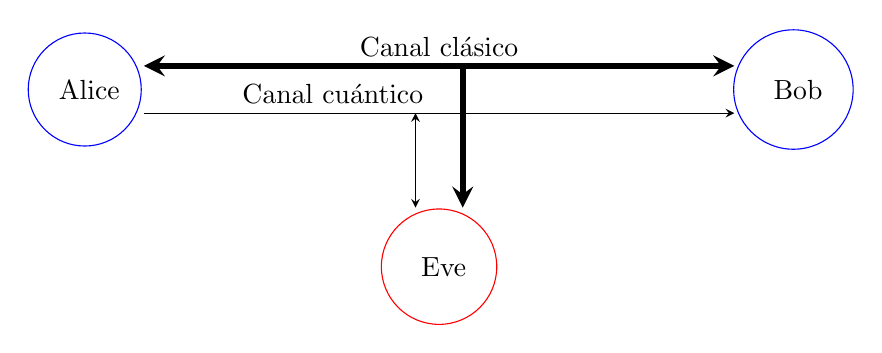
\begin{tikzpicture}[x=1.5cm, y=1.5cm]
    \node[circle,draw=blue] (v1) at (-3,0) {\ \ Alice\ \ };
    \node[circle,draw=blue] (v2) at (3,0) {\ \ \ Bob\ \ \ };
    \node[circle,draw=red] (v3) at (0,-1.5) {\ \ \ Eve\ \ \ };
    
    \draw[line width=0.8mm, {stealth}-{stealth}]  (-2.5,0.2) -- (2.5,0.2);
    \draw[line width=0.8mm, -{stealth}]  (0.2,0.2) -- (0.2,-1);
    
    \draw[-{stealth}]  (-2.5,-0.2) -- (2.5,-0.2);
    \draw[{stealth}-{stealth}]  (-0.2,-0.2) -- (-0.2,-1);
    
    \node at (0,0.2) [anchor=south] {Canal clásico};
    \node at (-0.9,-0.2) [anchor=south] {Canal cuántico};
\end{tikzpicture}
\end{center}
\caption{Esquema de distribución de clave cuántica.}
\label{fig:fig21}
\end{figure}

El primer paso del algoritmo es la elección de dos bases, como $\{\ket0,\ket1\}$ y $\{\ket+,\ket-\}$ y Alice procede a preparar una secuencia de bits. Para cada bit se elige aleatoriamente una de las bases para codificarlos, de manera que dicha codificación queda
\[\mathrm{bien\ }\begin{matrix}0\to\ket0\\1\to\ket1\end{matrix}\mathrm{,\ o\ bien\ }\begin{matrix}0\to\ket+\\1\to\ket-\end{matrix}\] 

en función de la base elegida. Tras la codificación, Alice envía a Bob la secuencia de qubits generada. Bob procede ahora a medir eligiendo, para cada qubit, una de las dos bases anteriormente citadas. Tras esta medición, tanto Alice como Bob hacen públicas las bases en las que la primera codificó y el segundo midió. Alrededor del 50\% de cada elección de estas bases coincidirá y los resultados asignados a estas elecciones se validan, mientras que el resto se desechan.

\begin{table}[htb]
\begin{tabular}{lll}
\rowcolor[HTML]{FFFFC7} 
Número del qubit & Base en la que codificó Alice & Base en la que midió Bob \\ 
\rowcolor[HTML]{FD6864} 
1                                & $\ket0,\ket1$                 & $\ket+,\ket-$            \\ 
\rowcolor[HTML]{9AFF99} 
2                                & $\ket0,\ket1$                 & $\ket0,\ket1$            \\ 
\rowcolor[HTML]{9AFF99} 
3                                & $\ket+,\ket-$                 & $\ket+,\ket-$            \\ 
\rowcolor[HTML]{FD6864} 
4                                & $\ket0,\ket1$                 & $\ket+,\ket-$            \\ 
\rowcolor[HTML]{9AFF99} 
5                                & $\ket+,\ket-$                 & $\ket+,\ket-$            \\ 
\rowcolor[HTML]{FD6864} 
6                                & $\ket+,\ket-$                 & $\ket0,\ket1$            \\ 
\rowcolor[HTML]{FD6864} 
7                                & $\ket+,\ket-$                 & $\ket0,\ket1$            \\ 
\rowcolor[HTML]{9AFF99} 
8                                & $\ket0,\ket1$                 & $\ket0,\ket1$            \\ 
\rowcolor[HTML]{9AFF99} 
9                                & $\ket0,\ket1$                 & $\ket0,\ket1$            \\ 
\rowcolor[HTML]{FD6864} 
10                               & $\ket0,\ket1$                 & $\ket+,\ket-$            \\ 
\rowcolor[HTML]{FFFFC7} 
...                              & ...                           & ...                      \\ 
\end{tabular}
\caption{Ejemplo de bases tomadas por Alice y Bob.}
\label{tab:tab21}
\end{table}

En el cuadro \ref{tab:tab21} se muestra un ejemplo de esta validación para los 10 primeros qubits de una secuencia. En verde aparecen los qubits para los que la base elegida por ambos coincidió y por tanto la medición de Bob arrojó el mismo resultado que la codificación de Alice. En rojo, por el contrario, aparecen aquellos cuyas bases no coincidieron y se descartan por no aportar información.

Ahora Alice y Bob pueden revelar una pequeña cantidad los valores obtenidos por cada uno, por ejemplo los $n$ primeros. Si todos esos valores coinciden, el canal es seguro y pueden utilizar el resto de los valores medidos no desvelados como clave. ¿Qué hubiera pasado si Eve hubiera intervenido el canal y hubiera tratado de medir los qubits antes de que lo hiciera Bob?

Al igual que Bob, Eve desconoce la base elegida por Alice para cada qubit, luego tendría que elegir una aleatoriamente  y realizar una medición. En el caso de escoger la misma que Alice (aunque Eve no podía tener la certeza hasta más tarde de haber acertado), no sólo podrá conocer el valor que codificó sino que además no está cambiando el estado del qubit y podrá reenviarlo a Bob inalterado. Esto ocurrirá en el 50\% de los casos; Sin embargo, en la otra mitad habrá elegido la base incorrecta modificando el estado del qubit y si Bob sí acierta con la base de Alice sólo tendrá un 50\% de posibilidades de medir el mismo valor que Alice codificó cuando debería serlo del 100\%.

Es así que Eve está introduciendo una variación en los estados en el 50\% de los qubits lo que supone que los valores de Alice y Bob diferirán en un 25\%. Si la cantidad de mediciones reveladas por ambos es de $n=20$ tras el intento de Eve de interceptar la comunicación, las probabilidades de no darse cuenta de la interferencia (no detectando ningún error) es de $0,75^{20}\approx0,32\%$. Tomando $n=30$ la probabilidad de pillar a Eve asciende a aproximadamente un 99,98\%, con lo que la certeza de garantizar la seguridad del canal es prácticamente absoluta con un tamaño de $n$ no necesariamente grande.

\section{Múltiples Qubits}

A lo largo de esta sección veremos cual es el comportamiento de un sistema cuántico cuando tenemos más de un qubit. Es aquí donde realmente podremos atisbar la capacidad de cómputo que tienen este tipo de máquinas.

En el física tradicional, si tenemos un sistema con $n$ partículas, cada una de ellas representada por un vector de dimensión 2, es el espacio vectorial que se genera es de dimensión $2n$. Esto se debe a que cada partícula se comporta de manera independiente y por tanto con ser capaces de modelizar el comportamiento individual de cada partícula tendremos representado todo el sistema. Es por ello que las dimensiones aumentan de manera lineal.

Sin embargo, esto no ocurre en mecánica cuántica. Las partículas ya no se comportan de manera independiente, si no que hay una dependencia entre ellas. Este efecto se llama \textbf{entrelazamiento} y entraremos en detalle posteriormente. 

Es por este motivo por el que no podemos modelizar los sistemas cuánticos con el comportamiento individual de cada partícula, si no que necesitaremos de una herramienta más potente, el \textbf{productor tensorial}.

\subsection{Producto Tensorial}

Supongamos que tenemos dos espacios vectoriales $\mathcal{V},\mathcal{W}$ de dimensiones $n$ y $m$ respectivamente. Entonces $\mathcal{V}\otimes\mathcal{W}$ es un espacio vectorial de dimension $n\times m$ y representa el producto tensorial de ambos espacios.

Además, supongamos que tenemos bases ortogonales para $\mathcal{V}$ y $\mathcal{W}$ dadas por:
\begin{equation}
\begin{split}
\mathcal{B}_v =\{\ket{v_i} |\ 1 \leq i \leq n \} \\
\mathcal{B}_w =\{\ket{w_j} |\ 1 \leq j \leq m \}
\end{split}
\end{equation}

Entonces una base $\mathcal{B}$ del espacio vectorial $\mathcal{V}\otimes\mathcal{W}$ se obtiene mediante el producto tensorial de los vectores de $\mathcal{B}_v$  y $\mathcal{B}_v$, es decir:
\begin{equation}
\mathcal{B} = \{\ket v\otimes\ket w|\ket v\in\B_v,\ket w\in\B_w\}
\end{equation}

Normalmente se aligera la notación y denotaremos $\ket{\phi}\otimes\ket{\psi}$ simplemente por $\ket{\phi}\ket{\psi}$ o incluso por $\ket{\phi\psi}$.

Por definición, el producto tensorial cumple las siguientes tres propiedades [\cite{nielsen2001quantum}]:
\begin{enumerate}
\item Dado un escalar z y un vector $\ket{v}$ de $\mathcal{V}$ y $\ket{w}$ de $\mathcal{W}$,\\
\begin{equation}
z(\ket{v}\otimes\ket{w})= (z\ket{v})\otimes\ket{w} = \ket{v}\otimes (z\ket{w})
\end{equation}

\item Para los vectores $\ket{v_1}$  y $\ket{v_2}$ de $\mathcal{V}$ y $\ket{w}$ de $\mathcal{W}$,\\
\begin{equation}
(\ket{v_1}+\ket{v_2})\otimes\ket{w}=\ket{v_1}\otimes\ket{w}+\ket{v_2}\otimes\ket{w}
\end{equation}

\item Para los vectores $\ket{v}$ de $\mathcal{V}$ y $\ket{w_1}$, $\ket{w_2}$ de $\mathcal{W}$,\\
\begin{equation}
\ket{v}\otimes (\ket{w_1}+\ket{w_2}) = \ket{v}\otimes\ket{w_1} +\ket{v}\otimes\ket{w_2} 
\end{equation}
\end{enumerate}

Hemos visto el producto tensorial aplicado a espacios vectoriales y hemos definido las propiedades que debe verificar un operador para ser considerado tensorial. Veamos cómo aplicaremos este operador en el caso de vectores, aunque lo haremos de una manera más general, definiendo el producto tensorial entre matrices. No olvidemos que un vector tiene una representación matricial como columna.

Sean $A$ y $B$ matrices con coeficientes complejos de dimensiones $m\times n$ y $p\times q$ respectivamente. Se verifica

\begin{equation}
A\otimes B=\left(\begin{matrix}
a_{11}B & \hdots & a_{1n}B \\
\vdots & \ddots & \vdots \\
a_{m1}B & \hdots & a_{mn}B
\end{matrix}\right)
\end{equation}

lo que supone que la matriz resultante $A\otimes B$ tiene dimensiones $mp\times nq$. Así, sean dos qubits, cuyos espacios vectoriales están representados respectivamente por la base ortonormal estándar $\{\ket0,\ket1\}$. Entonces, el nuevo espacio vectorial 
generado por ambos qubits tiene como base los vectores $\{\ket{00},\ket{01},\ket{10},\ket{11}\}$, es decir, un espacio de dimensión 4. Sin embargo, este ejemplo no es demasiado ilustrativo (pues $2^n = 2n$ si $n=4$).

Así que supongamos que añadimos un tercer qubit a nuestro sistema de dos qubits. Entonces el nuevo espacio vectorial tendrá dimensión 8 ($2^3$) y su base viene dada por los vectores $\{\ket{000},\ket{001},\ket{010},\ket{011},\ket{100},\ket{101},\ket{110},\ket{111}\}$.

Pero recordemos que un qubit tiene también una representación como vector columna, y por lo tanto podemos aprovecharnos de dicha representación para calcular  productos tensoriales entre qubits.

Supongamos que tenemos dos qubits $\ket{\psi}$ y $\ket{\phi}$ que cumplen:\\
\begin{equation}
\begin{split}
\ket{\psi}=a\ket0+b\ket1,\ |a|^2 + |b|^2 = 1\\
\ket{\phi}=c\ket0+d\ket1,\ |c|^2 + |d|^2 = 1
\end{split}
\end{equation}

Estos qubits se pueden ver en forma de matriz como:
\begin{equation}
\begin{split}
\ket{\psi} = \twovector{a}{b}\\
\ket{\phi} = \twovector{c}{d}
\end{split}
\end{equation}

Y por tanto, esta representación nos permite calcular el producto tensorial $\ket{\psi}\otimes\ket{\phi}$ como:
\begin{equation}
\ket{\psi}\otimes\ket{\phi} = \twovector{a}{b}\otimes\twovector{c}{d} = \begin{pmatrix} ac \\ ad \\ bc \\ bd  \end{pmatrix}
\end{equation}

Recuperando la notación de Dirac, este vector sería $\ket{\psi}\otimes\ket{\phi} = ac\ket{00} + ad\ket{01} + bc\ket{10} + bd\ket{11}$. De esta forma, se ha obtenido un vector de dimensión 4 que, además, sigue cumpliendo la restricción de normalización ya que:
\begin{equation}
\begin{split}
 |ac|^2 + |ad|^2 + |bc|^2 + |bd|^2 =\\ |a|^2|c|^2 + |a|^2|d|^2 + |b|^2|c|^2 + |b|^2|d|^2 =\\ |a|^2(|c|^2 + |d|^2) + |b|^2(|c|^2 + |d|^2) =\\ |a|^2 + |b|^2 = 1
\end{split}
\end{equation}

Una vez que hemos visto como operar qubits mediante el producto tensorial es imprescindible mostrar que existen ciertos estados cuánticos que no se pueden expresar mediante el producto tensorial. Este tipo de estados son conocidos como \textbf{estados entrelazados}. Un ejemplo de este tipo de estados es el dado por $\ket{00} + \ket{11}$. Veamos que efectivamente no se puede obtener dicho estado mediante el producto tensorial de dos qubits.

Supongamos que dichos qubits si que existen. Entonces tenemos:
\begin{equation}
(a\ket0 + b\ket1)\otimes (c\ket0 + d\ket1) = \ket{00} + \ket{11}
\end{equation}
Además, por lo visto anteriormente se tiene también que:
\begin{equation}
(a\ket0 + b\ket1)\otimes (c\ket0 + d\ket1) = ac\ket{00} + ad\ket{01} + bc\ket{10} + bd\ket{11}
\end{equation}
Y por tanto, los miembros de la derecha de ambas ecuaciones deben ser igual. Para ello se debe cumplir que $ ad = 0$ y $bc=0$. Sin embargo, si alguno de los coeficientes $a,\ b,\ c,\ d$ es cero, anularía  también la amplitud correspondiente al estado $\ket{00}$ o $\ket{11}$ según corresponda, y esto es absurdo.

Este tipo de estados no guardan similitud alguna con el mundo clásico, y son los causantes de aportar el crecimiento exponencial respecto del número de partículas en el sistema.

Por último, queda ver qué ocurre con las mediciones en un sistema con múltiples qubits. Supongamos que tenemos un estado general en un sistema de 2 qubits dado por:
\begin{equation}
a\ket{00} + b\ket{01} + c\ket{10} + d\ket{11}, 
\end{equation}

donde $a,\ b,\ c,\ d$ son números complejos que cumplen la restricción de normalización: $|a|^2 + |b|^2 + |c|^2 + |d|^2 = 1$.

Si medimos el primer qubit respecto de la base estándar $\{\ket0,\ket1\}$, se obtendrá $\ket0$ con una probabilidad $|a|^2 + |b|^2$ y $\ket1$ con probabilidad $|c|^2 + |d|^2$. Además si se obtiene $\ket0$ al medir el primer qubit, el estado colapsa al subespacio compatible con la medida, es decir, al generado por los vectores $\ket{00}$ y $\ket{01}$. De esta forma se proyectaría el sistema al estado  $a\ket{00} + b\ket{01}$ tras realizar una primera medición. Sin embargo, este estado no está normalizado, luego realmente se obtendría el estado: 
\begin{equation}
\dfrac{1}{\sqrt{|a|^2 + |b|^2}}(a\ket{00} + b\ket{01})
\end{equation}

En este nuevo estado tendríamos por lo tanto que al realizar una medida sobre el segundo qubit, obtenemos con probabilidad $|a|^2$ el estado $\ket0$, mientras que  $\ket1$ se obtiene con probabilidad $|b|^2$.

Es muy particular las mediciones en estados entrelazados, ya que, como se muestra a continuación, realizar una medición sobre uno de los qubits influye en el estado de los otros.

Dado el estado entrelazado $\tfrac{1}{\sqrt{2}}(\ket{00} + \ket{11})$ es claro que es equiprobable obtener el estado $\ket0$ o $\ket1$ al realizar una medida sobre el primer qubit. Sin embargo, si el segundo qubit ya ha sido medido previamente, y por ejemplo se ha obtenido el estado $\ket0$, entonces el sistema colpasará al estado $\ket{00}$, y en este nuevo estado se obtiene con probabilidad 1 el estado $\ket0$ al medir el primer qubit. Esta propiedad de los estados entrelazados es en la que se basan algunos de los experimentos más relevantes de la computación cuántica, como puede ser el experimento de \textit{teleportación} o \textit{codificación densa}. 

Una vez visto como actúan múltiples qubits dentro de un sistema, a lo largo de la siguiente sección se desarrollará con detalle como aplicar la principal herramienta que permite modificar el estado de los qubits: las puertas cuánticas.

\section{Puertas cuánticas}

En computación clásica los bits son operados mediante una serie de puertas que son representadas como un circuito cableado. De igual modo tenemos puertas en el mundo cuántico. Dichas puertas tienen que verificar ser isomorfismos lineales unitarios; es decir, Si $U$ es la matriz asociada de dicho isomorfismo, se debe verificar que

\begin{equation}
UU^*=I
\end{equation}

donde $U^*$ es la matriz conjugada traspuesta de $U$. Una consecuencia inmediata de esta igualdad es que cualquier puerta cuántica es reversible, cosa que no ocurría con las clásicas. Además, por ser isomorfismo, el número de qubits de entrada coincidirá con el de salida.

\subsection{Puerta cuánticas de un qubit}

Vamos a proceder a hablar de algunas de las puertas cuánticas que cuentan con un solo qubit de entrada y salida más relevantes. Mostraremos la transformación realizada por cada una de ellas sobre los elementos de la base $\{\ket0,\ket1\}$, su expresión matricial y cómo se representan gráficamente sobre un circuito.

\[\begin{matrix}
\gatetwo{I}{\ket0}{\ket1} & \left(\begin{matrix}1&0\\0&1\end{matrix}\right) & \Qcircuit @C=1em @R=.7em {& \gate{I} & \qw}\\
\gatetwo{X}{\ket1}{\ket0} & \left(\begin{matrix}0&1\\1&0\end{matrix}\right) & \Qcircuit @C=1em @R=.7em {& \gate{X} & \qw}\\
\gatetwo{Y}{-\ket1}{\ket0} & \left(\begin{matrix}0&1\\-1&0\end{matrix}\right) & \Qcircuit @C=1em @R=.7em {& \gate{Y} & \qw}\\
\gatetwo{Z}{\ket0}{-\ket1} & \left(\begin{matrix}1&0\\0&-1\end{matrix}\right) & \Qcircuit @C=1em @R=.7em {& \gate{Z} & \qw}\\
\end{matrix}\]

Estas cuatro puertas son denominadas \textbf{puertas de \textit{Pauli}}. La primera de ellas se trata de la identidad que deja un estado cuántico invariable. $X$ es la puerta negación, dado un qubit $\ket\psi=\alpha\ket0+\beta\ket1$, tenemos que $X(\ket\psi)=\beta\ket0+\alpha\ket1$. $Z$ aplica un cambio de fase sobre $\ket1$ pero no varía las amplitudes (y por tanto tampoco las probabilidades de obtener $\ket0$ o $\ket1$ aplicando una medición). Por último, $Y$ es combinación de $X$ y $Z$ ($Y=ZX$).

Existen otras puertas de cambio de fase como $Z$ que denotamos de manera general por:

\[\begin{matrix}
\gatetwo{R_\theta}{\ket0}{e^{i\theta}\ket1} & \left(\begin{matrix}1&0\\0&e^{i\theta}\end{matrix}\right) & \Qcircuit @C=1em @R=.7em {& \gate{R_\theta}& \qw}
\end{matrix}\]

Nótese que $R_\pi=Z$. La puerta más relevante que veremos en esta sección es la \textbf{Puerta de \textit{Hadamard}}. Esta puerta es importante puesto que nos permite conseguir un estado en superposición de manera que las amplitudes de $\ket0$ y $\ket1$ produzcan equiprobabilidad en la medición. La describimos como:

\[\begin{matrix}
\gatetwo{H}{\dfrac{1}{\sqrt{2}}(\ket0+\ket1)}{\dfrac{1}{\sqrt{2}}(\ket0-\ket1)} & \left(\begin{matrix}\dfrac{1}{\sqrt{2}}&\dfrac{1}{\sqrt{2}}\\\dfrac{1}{\sqrt{2}}&-\dfrac{1}{\sqrt{2}}\end{matrix}\right) & \Qcircuit @C=1em @R=.7em {& \gate{H}& \qw}
\end{matrix}\]

Si esta puerta se aplica individualmente a cada uno de los $n$ qubits de un sistema con estado inicial $\ket{0\hdots0}$ obtenemos:

\begin{equation}
\dfrac{1}{\sqrt{2}}(\ket0+\ket1)\otimes\hdots\otimes\dfrac{1}{\sqrt{2}}(\ket0+\ket1)=\dfrac{1}{\sqrt{2^n}}\sum_{i=1}^{2^n-1}\ket i
\end{equation}

Esta última igualdad nos da una idea del poder que puede alcanzar el cómputo cuántico, pues hemos obtenido $2^n$ estados distintos en superposición. Cuando aplicamos la puerta de \textit{Hadamard} sobre $n$ qubits la denominamos \textbf{puerta de \textit{Walsh-Hadamard}} definida recursivamente como:

\[\begin{matrix}W_1=H,&W_{n+1}=H\otimes W_n\end{matrix}\]

En la figura \ref{fig:fig22} podemos ver un ejemplo sencillo de la aplicación de la puerta de \textit{Hadamard} sobre los 4 qubits de un sistema cuántico (o equivalentemente la aplicación de la puerta $W_4$). El estado del sistema tras la aplicación de dichas puertas es de 

\[\ket\psi=\dfrac{1}{4}\sum_{i=0}^{15}\ket i.\]

\begin{figure}[!htb]
\[\Qcircuit @C=1em @R=.7em {
\lstick{\ket{0}} & \qw & \qw & \gate{H} & \qw & \qw & \qw \\
\lstick{\ket{0}} & \qw & \qw & \gate{H} & \qw & \qw & \qw \\
\lstick{\ket{0}} & \qw & \qw & \gate{H} & \qw & \qw & \qw \\
\lstick{\ket{0}} & \qw & \qw & \gate{H} & \qw & \qw & \qw
}\]
\caption{Puertas de \textit{Hadamard} aplicadas a un sistema de 4 qubits.}
\label{fig:fig22}
\end{figure}

\subsection{Puertas cuánticas de más de un qubit}

La puerta de \textit{Walsh-Hadamard} está definida para más de un qubit; Sin embargo, puede ser expresada con producto tensorial de varias puertas de un solo qubit. No es el caso de las puertas que veremos en esta sección. En primer lugar presentamos la puerta \textbf{\textit{SWAP}} cuya función es intercambiar los estados de dos qubits. Su representación matricial es

\[\left(\begin{matrix}1&0&0&0\\0&0&1&0\\0&1&0&0\\0&0&0&1\end{matrix}\right)\mathrm{\ y\ en\ circuitos\ se\ representa\ como\ }
\Qcircuit @C=1em @R=1em {
& \qswap & \qw \\
& \qswap \qwx & \qw
}.\]

Un grupo de puertas de dos qubits muy relevante es el de las \textbf{puertas controladas}. Su funcionamiento consiste en tomar un primer qubit como control que permanecerá inalterado y un segundo al que se le aplicará una puerta $U$ o no en función del estado del primero. Su representación matricial por bloques viene dada por

\[C(U)=\left(\begin{array}{c|c}I&0\\\hline0&U\end{array}\right).\]

La más importante de ellas es $C(X)$, más conocida como \textbf{\textit{CNOT}} descrita por:

\[\begin{matrix}
\gatefour{\mathrm{CNOT}}{\ket{00}}{\ket{01}}{\ket{11}}{\ket{10}} & \left(\begin{matrix}1&0&0&0\\0&1&0&0\\0&0&0&1\\0&0&1&0\end{matrix}\right) & \Qcircuit @C=1em @R=1em {& \ctrl{1} & \qw \\
& \targ & \qw}
\end{matrix}\]

donde $\bullet$ denota el qubit de control y $\oplus$ el qubit negado (si procede). Como vemos, la puerta $X$ se aplica sobre el segundo qubit si el estado del primero es $\ket1$.

Existen puertas controladas en las que intervienen más de dos qubits como la \textbf{\textit{CCNOT}} o \textbf{puerta de \textit{Toffoli}}. Se trata de una puerta de 3 qubits, los dos primeros de control que permanecen inalterados y el último al que se le aplica una puerta $X$ siempre y cuando los dos primeros sean $\ket1$. Para simplificar, mostramos su matriz por bloques y su representación en circuito:

\[\begin{matrix}
T=\left(\begin{array}{c|c|c}I&0&0\\\hline0&I&0\\\hline0&0&X\end{array}\right) & \Qcircuit @C=1em @R=1em {& \ctrl{1} & \qw \\
& \ctrl{1} & \qw \\
& \targ & \qw}
\end{matrix}\]

Esta puerta tiene una importancia adicional porque con ella podemos emular las puertas clásicas \textbf{NOT} y \textbf{AND} que constituyen un conjunto universal que permiten construir cualquier circuito clásico.

\begin{equation}
\begin{split}
T\ket{1,1,x}=\ket{1,1,\neg x} \\
T\ket{x,y,0}=\ket{x,y,x\wedge y}
\end{split}
\end{equation}

En la ecuación anterior se muestran las construcciones de dichas puertas respectivamente. Nótese que $T$ permite generar cualquier circuito clásico pero no afirmamos tal cosa de los circuitos cuánticos (de hecho no se verifica esta segunda proposición). La generación de estas puertas ayudó a probar a Deutsch que cualquier función clásica puede ser fabricada a partir de una puerta cuántica reversible [\cite{deutsch1985quantum}]. Incluso Bernstein y Vazirani concretaron una \textbf{máquina cuántica universal de Turing} [\cite{bernstein1997quantum}].

Según lo que acabamos de ver, dada una función clásica $\function{f}{\{0,1\}^m}{\{0,1\}^k}$ existe un \textbf{\textit{array} de puertas} $U_f$ que implementa $f$ en un circuito cuántico. Se verifica que $U_f\ket{x,y}=\ket{x,y\oplus f(x)}$ donde $x$ denota un elemento de $m$ bits, $y$ de $k$ bits y $\oplus$ es el operador lógico XOR.

\begin{figure}[!htb]
\[\Qcircuit @C=1em @R=.7em {
\lstick{\ket{x}}& \multigate{1}{U_f} & \qw & \qw & \qw & \qw & & \lstick{\ket{x}} \\
\lstick{\ket{y}}& \ghost{U_f}        & \qw &     &     &     & & \lstick{\ket{y\oplus f(x)}}
}\]
\caption{Representación en un circuito cuántico de un \textit{array} de puertas cuántico.}
\label{fig:fig23}
\end{figure}

Véase que $U_fU_f\ket{x,y}=U_f\ket{x,y\oplus f(x)}=\ket{x,y\oplus f(x)\oplus f(x)}=\ket{x,y}$. Luego $U_fU_f=I$ y por lo tanto verifica que es unitaria. Para calcular $f(x)$ basta con aplicar $U_f\ket{x,0\hdots0}$ cuyo resultado será $\ket{x,f(x)}$.

Sin embargo esto no parece suponer una gran ventaja respecto la computación clásica. Pero, ¿y si pudiéramos obtener todos los valores $f(x)$ para cada $x\in\{0,1\}^m$ con una sola aplicación de $U_f$? Esto constituye una mejora de complejidad exponencial a constante y lo conseguimos aplicando una puerta de \textit{Hadamard} a cada uno de un total de $m$ qubits (es decir, aplicar $W_m$), además de preparar otros $k$ qubits en estado $\ket0$ tal y como muestra la figura \ref{fig:fig24}.

\begin{figure}[!htb]
\[\Qcircuit @C=1em @R=.7em {
\lstick{\ket{0\overset{m}\hdots0}}& \gate{W_m} & \multigate{1}{U_f} & \qw \\
\lstick{\ket{0\overset{k}\hdots0}}& \qw        & \ghost{U_f}        & \qw
}\]
\caption{Ejemplo del poder del paralelismo cuántico aplicado a un \textit{array} de puertas.}
\label{fig:fig24}
\end{figure}

Analíticamente, por la linealidad de $U_f$, tenemos:

\begin{equation}
\begin{split}
U_f(W_m(\ket{0\overset{m}\hdots0})\otimes\ket{0\overset{k}\hdots0})&=U_f\left(\dfrac{1}{\sqrt{2^m}}\sum^{2^m-1}_{i=0}\ket{i,0\overset{k}\hdots0}\right)=\\
&=\dfrac{1}{\sqrt{2^m}}\sum^{2^m-1}_{i=0}U_f\ket{i,0\overset{k}\hdots0}=\dfrac{1}{\sqrt{2^m}}\sum^{2^m-1}_{i=0}\ket{i,f(i)}
\end{split}
\end{equation}

No obstante, todo esto no es tan maravilloso como parece. Recordemos que sólo podemos obtener información de un estado cuántico mediante la medición y, que tras esta, el estado que obtengamos será el mismo al que colapsará el sistema y será único, con lo que perdemos este poder de \textbf{paralelismo cuántico} que acabábamos de obtener. Antes de medir, debemos aplicar algunas técnicas adicionales, alejadas de la computación clásica como por ejemplo amplificar las amplitudes (y con ellas las probabilidades de medir ese estado) de los valores de mayor interés.

\subsection{Teorema de no clonación}

\begin{thm} \textbf{Teorema de no clonación}
Dado un estado cuántico desconocido $\ket{\phi}$ es imposible realizar una copia de dicho estado mediante transformaciones unitarias.
\end{thm}

Supongamos que pudiéramos construir una maquina cuántica capaz de clonar estados cuánticos mediante transformaciones unitarias. Es decir, que existe un operador unitario $U$  tal que :
\begin{equation}
U(\ket{\phi 0}) = \ket{\phi\phi} \textrm{, para cualquier estado } \ket\phi 
\end{equation}

Supongamos ahora que tenemos un estado ortogonal a $\phi$ que denotaremos por $\psi$. Esto nos permite definir un tercer estado como superposición de los dos anteriores. Dicho estado viene dado por:
\begin{equation}
\ket\Psi = \dfrac{1}{\sqrt{2}}(\ket\phi + \ket\psi)
\end{equation}

Si aplicamos el operador lineal $U$ al estado $\Psi$ se obtiene:
\begin{equation}
U(\ket{\Psi 0})= \dfrac{1}{\sqrt{2}}(U\ket{\phi 0} + U\ket{\psi 0}) = \dfrac{1}{\sqrt{2}}(\ket{\phi\phi} + \ket{\psi\psi})
\end{equation}

Sin embargo, como este operador es el operador de clonación, también se tiene:
\begin{equation}
U(\ket{\Psi 0})= \ket{\Psi\Psi} = \dfrac{1}{2}(\ket{\phi\phi} + \ket{\phi\psi} + \ket{\psi\phi} + \ket{\psi\psi})
\end{equation}

Como los lados derechos de las dos ecuaciones anteriores no son iguales, se sigue el resultado. No existe una operación unitaria que pueda clonar un estado cuántico desconocido.